
% SECTION : layer_1_physical {{{
\section{Layer 1 : Physical}
\label{sec:layer_1_physical}
\parindent=0em

Layer 1, the Physical Layer

This layer deals with the hardware of networks such as cabling. It defines the mechanical and electrical standards of interface devices and the types of cables used to transmit digital signals (e.g. optical fiber, coaxial cable, wireless, etc.).

The major protocols used by this layer include Bluetooth, PON, OTN, DSL, IEEE.802.11, IEEE.802.3, L431 and TIA 449.


Latency is the term used to describe the total time it takes a data packet to
travel from one node to another. This is often measured in milliseconds (ms).
The greater the latency, or "lag," the higher this number will be.

Availability refers to how long the network stays up and operational without
interruption, and how quickly it can recover should it go down.

Bandwidth refers to the maximum amount of data that can be transmitted over a
medium in a given time.

Throughput refers to the actual amount of data that is transmitted over a medium
in a given time.

% 	SUB-SECTION : telephony {{{
\subsection{Telephony}
\label{ssec:telephony}


% packet switching {{{


A TCP/IP network transmits data to the desired recipient using packet switching.
To accomplish this, each packet of information has a source and destination
address. A router is responsible for analyzing the packet header information and
directing the packet based on pre-configured tables.

Frame Relay Line

ATM ( Asynchronus Transfer Mode )

MPLS ( Multiprotocol Label Switching )

% }}}

% circuit switching {{{

% }}}

CSU / DSU : converts LAN data to WAN data

Patch Panel

110 Block


% 		SUB-SUB-SECTION : sonet {{{
\subsubsection{SONET}
\label{sssec:sonet}


SONET : Synchronus optical Networking. These are the optical equivalents of T1
lines and are called OC-Lines. The signal types (basically just the frame type)
used in these lines is called STS. Each consequtive line is essentially a
mutiple of 52 making the following table a lot easier to remember.

OC-1   : 51.85 Mbps  : STS-1
OC-3   : 155.52 Mbps : STS-3
OC-12  : 622.08 Mbps : STS-12
OC-24  : 1.244 Gbps  : STS-24
OC-48  : 2.488 Gbps  : STS-48
OC-192 : 9.955 Gbps  : STS-192
OC-256 : 13.22 Gbps  : STS-256
OC-768 : 39.82 Gbps  : STS-768

DWDM

\subsubsectionend
% }}} END SUB-SUB-SECTION : sonet

% 		SUB-SUB-SECTION : trunk_lines {{{
\subsubsection{Trunk Lines}
\label{sssec:trunk_lines}

analog signal

digital signal

fdm ( frequency division multiplexing ) : Origianl telphone systems used
frequency division multiplexing , today they use time division multiplexing.

tdm ( time division multiplexing )

DS0 Signal

DS1 Signal : A DS1 Signal is 24 DS0 signals all going down the same wire.

DS3 Signal :


T1 Cable Line : 24 channels , 1.544 Mbps
T3 Cable Line : 672 Channels , 44.736 Mbps
E1 Cable Line : 32 , 2.048 Mbps
E3 Cable Line : 512 , 34.368 Mbps

T1 Crossover

PSTN ( Public Switched Telephone Network )

Dial-Up : Provided by telephone lines. To connect to the internet , you would
get a connection line through your dial-up ISP. This means that the ISP would
give you a telephone number , username and password. You call this telephone
number from your modem through your computer. Dial-up uses the PPP protocol. Be
careful when thinking about the timeline though , cause dial-up refers to the
phone line which came about decades before dial-up networking.

BPL (Broadband over power line) : This is basically a technology that uses power
lines to deliver internet in addition to electricity. Not very successful in
terms of implementation and is rare to find. The main problem was the huge
amount of interference due to electricity while running on the same line. This
was in addition to the danger of having to make patches and stuff cause the wire
was carrying not only a signal but also live current.

\subsubsectionend
% }}} END SUB-SUB-SECTION : trunk_lines

% 		SUB-SUB-SECTION : isdn {{{
\subsubsection{ISDN}
\label{sssec:isdn}


ISDN ( Integrated Service Digital Network ) : Came up before dial-up networking
and provided either 64Kbps or 128 Kbps speeds. These used ISDN phones , and you
would also get a ISDN adapter that you would plug into to be able to get
connected.

\subsubsectionend
% }}} END SUB-SUB-SECTION : isdn

% 		SUB-SUB-SECTION : pbx {{{
\subsubsection{PBX}
\label{sssec:pbx}



\subsubsectionend
% }}} END SUB-SUB-SECTION : pbx

% 		SUB-SUB-SECTION : voip {{{
\subsubsection{VoIP}
\label{sssec:voip}

RTP
STRP
RDP
Kubernetes

RTP : udp 5004 / udp 5005
RTSP
SIP : tcp 5060 / 5061
H.323 : tcp 1720
MGCP : 2427 / 2727 , Media Gateway Control Protocol


\subsubsectionend
% }}} END SUB-SUB-SECTION : voip


\subsectionend
% }}} END SUB-SECTION : telephony

% 	SUB-SECTION : 802_3_ethernet {{{
\subsection{802.3 : Ethernet}
\label{ssec:802_3_ethernet}

POE : Power over Ethernet . Back in the day you would need to give WAPs two
seperate sets of input. One would be the ethernet input , the other would be
power input so that the device had electricity to function. Today we can provide
power over the ethernet cable itself. This is called POE. This is used in
difficult to power areas. It is commonly used with phones, wireless access
points and cameras. The power is usually comming directly from the switch that
the ethernet cable is plugged into. This is called an endspan. If the switch
does not provide power , then a power injector is installed in the middle. This
type of connection is called a Midspan.

802.3af , PoE : 15.4 watts
802.3at , PoE+ : 30 watts

EOP : ethernet over power is the reverse of POE. This allows us to extend our
ethernet network using the power cables that we already have in our homes. This
is also called PLC (Power line communication). These types of connections can
deliver 500 Mbps. Commonly only devices that are not traditionally connected to
the internet use these connections. An example is electric cars, which can
charge and be connected to the internet through EOP.

\subsectionend
% }}} END SUB-SECTION : 802_3_ethernet

% 	SUB-SECTION : 802_11_wireless {{{
\subsection{802.11 : Wireless}
\label{ssec:802_11_wireless}

802.11 is a IEEE Protocol that uses radio waves to transfer network information
between different individual wireless nodes.

Wireless Bridge : A normal bridge is one that joins two networks so that they
can work together as one larger network. A Wireless bridge does the same with
wireless networks. There can be more than one type of wireless bridge however :

- Wi-Fi to Ethernet Bridge : Usually WAP to Ethernet
- Wi-Fi to Wi-Fi : Joins two wireless networks usually to increase coverage.
- Bluetooth to Wi-fi Bridge : Allows connecting to Wi-Fi through bluetooth.

Wi-Fi Repeater Mode is a variation on bridging. Rather than connect seperate
netowrks in a way that allows devices in each one to communicate with each
other, repeater mode extends the wireless signal of one network to longer
distances.

Wireless Range Extenders basically work as Wi-Fi Repeaters.

SSID (Service Set Identifier) : Each WAP has a word or a phrase that is used to
help wireless devices identify and connect to the WAP. These words / phrases are
called SSIDs and are typically broadcasted to whoever wants to attempt to
connect to them.

BSSID ( Basic Service Set Identifier )
ESSID ( Extended Service Set Identifier )

Infrastructure Mode

Ad Hoc Mode

Wireless Bands : A band is a range of frequencies across the electromagnetic
spectrum. Basically the electromagnetic spectrum (radio , micro, infrared ,
visiable , ultravoilet , x-rays , gamma rays) is first chopped up according to
wavelength. Then within each wavelenth people decide to further break up the
spectrum into smaller ranges called bands.  So different technologies with
different ranges , power needs , applications etc ... will use different bands
in different wavelengths throughout the EM Spectrum.

Wireless Channel : Which in turn are broken again into smaller units called
channels.So channels are individual , smaller sections of the overall frequency
band used by a wireless network. The width of the these channels is usually
measure in MHz and is called the channel width. Channel also have something
called a channel buffer , which is a empty frequency space put around channels
widths in a band since radiowaves are imperfect and we want to allow for some
fluctuations without overlap. Each channel is marked using the center of the
channel width.  As an example if we have a channel in the 2.4Ghz band going from
2.4Ghz to 2.42Ghz , with channel width 22MHz , we have channel midpoints : 2.412
, 2.437 , 2.462. These 3 channels in the 2.4 band are called channels 1 , 3 and
7.  These are the conly channels we can have without overlap.

ISM Bands : All 802.11 networks are designed to run in the industrial ,
scientific and medical bands. These are portions of the radio spectrum that are
reserved internationally for telecommunication communication purposes.  Although
for 802.11 these days we will primarily only deal with 2 bands : 2.4/5.0GHz.
This means that these 2.4Ghz and 5.0Ghz are the starting points for the bands
that these technologies use. So the 2.4Ghz band will use 2.40Ghz to roughly
2.5Ghz as its band range, and within this band we will have multiple channels
specified in MHz. Disributing the number and size of a channel usually depends
on the regulatory commitee in specific countries.

CSMA / CA : When we try to get two machines to communicate with each other using
wireless radio waves , we very quickly will run into a problem. The problem
being that what if multiple devices are talking on the same channel. This
causes interference , and is very similar to the early days of the ethernet
where the NICs would detect collisions on the wired networks before we had
switches. The wireless solution to this is called Carrier Sense Multiple Access
Collision Avoidance or CSMA / CA. Do not confuse this with CSMA / CD which is
the wired ethernet equivalent. CSMA will basically only allow communications
between a client and a server to take place as long as the coast is clear. This
ensures that there are never any collisions because they avoid each other and do
not even try to communicate until a channel is open and free.

DSSS ( Digital-sequence spread-spectrum ) : 

OFDM ( Orthogonal frquency-division multiplexing )

Wireless Controller : When we have several WAPs working together , we do not
want to go and configure each one individually. In this case we use a device
called a wireless controller which allows us to configure all of the WAPs at the
same time by propogating out the changes to all the devices.

% TABULAR TABLE : 802_11_bands {{{

\begin{figure*}[ht]
\centering

\tabulartable
{0.99\linewidth}
{t}
{c|ccccc}
{

802.11a  & 54Mbps        & 5.0GHz     & 20MHz & OFDM & \\
802.11b  & 11Mbps        & 2.4GHz     & 22MHz & DSSS & \\
802.11g  & 54Mbps        & 2.4GHz     & 20MHz & OFDM & \\
802.11n  & 108 - 300Mbps & 2.4/5.0GHz & 20MHz/40MHz & OFDM & MIMO \\
802.11ac & 1Gbps +       & 5.0GHz     & 160MHz & OFDM & MU-MIMO \\

}

\caption{802.11 Extension Evolution}
\end{figure*}

% }}} End TABLE : 802.11 Bands

% 		SUB-SUB-SECTION : antennas {{{
\subsubsection{Antennas}
\label{sssec:antennas}

Omni Antenna
\begin{figure}[h!]
  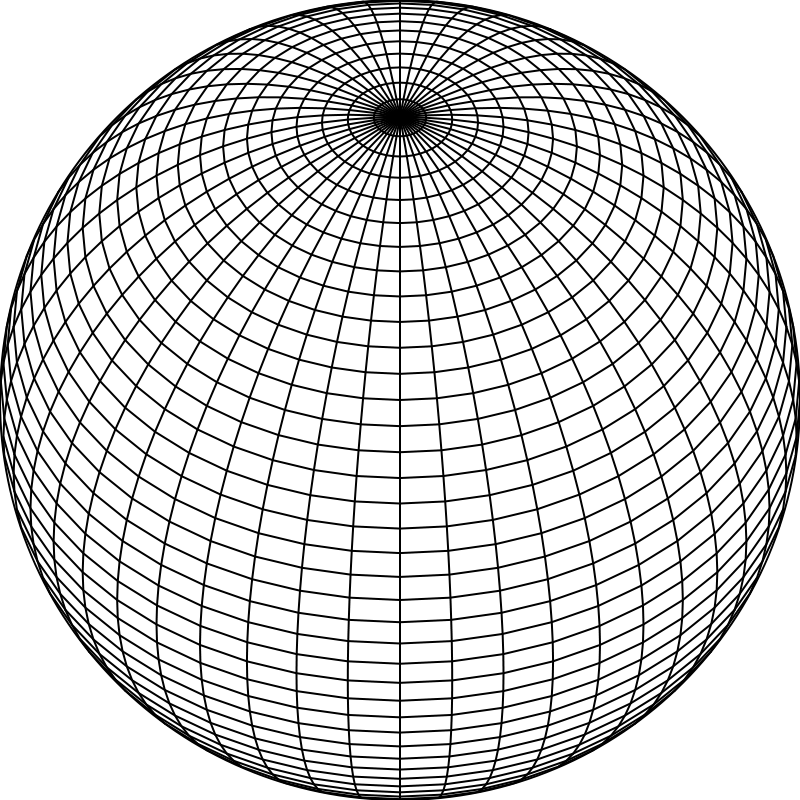
\includegraphics[width=\linewidth]{omni_antenna.png}
  \caption{Omnipole Antenna Pattern.}
  \label{fig:placeholder}
\end{figure}





Dipole Antenna
\begin{figure}[h!]
  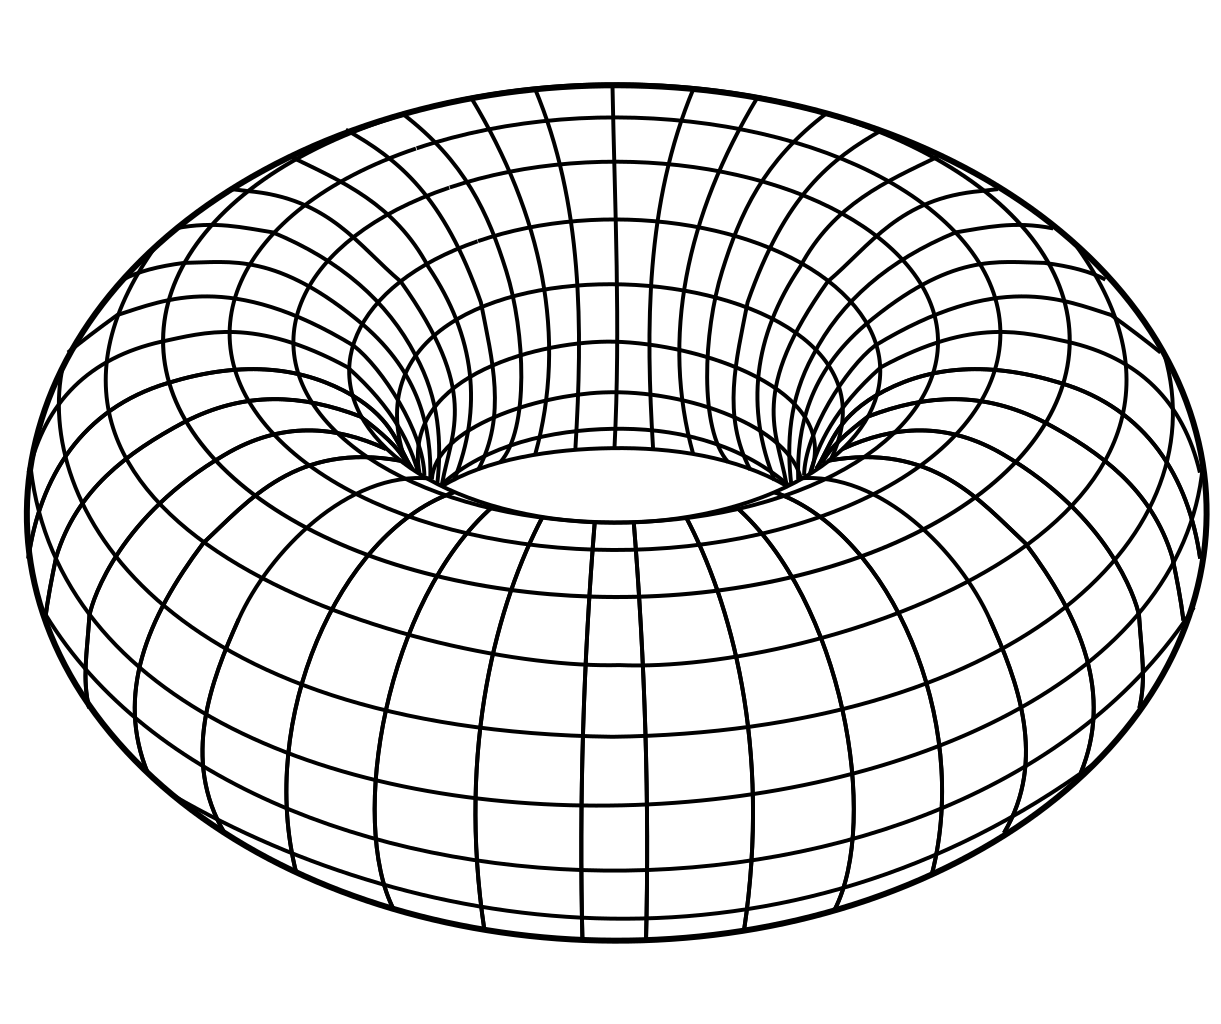
\includegraphics[width=\linewidth]{dipole_antenna.png}
  \caption{Dipole Antenna Pattern.}
  \label{fig:placeholder}
\end{figure}


\begin{figure}[h!]
  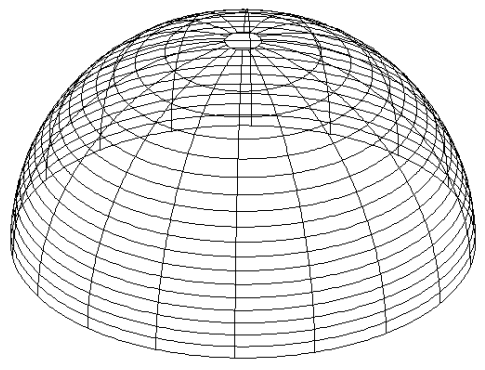
\includegraphics[width=\linewidth]{patch_antenna.png}
  \caption{Patch Antenna Pattern.}
  \label{fig:placeholder}
\end{figure}

Directional Antenna / Yagi Antenna

Parabolic Antenna

SMA Connector

Antenna Gain : Measured in dBi
\subsubsectionend
% }}} END SUB-SUB-SECTION : antennas

% 		SUB-SUB-SECTION : 802_11_coverage {{{
\subsubsection{802.11 Coverage}
\label{sssec:802_11_coverage}


Reflection : This is when the radio waves are bounding off the surface and
travelling in roughly the opposite direction of what they came in. If we have
rooms / offices behind materials like metal walls , then the radio waves will
get strondly reflected by the wall and it would be difficult for them to
connect.

Refraction : In opposition to reflection , refraction bends the radio waves only
a little bit such that their trajectory changes. Certain materials like glass
walls can cause the radio waves to bend in another direction than the one in
which they were intially intended to travel. This can be used to our advantage
however.

Absorbtion : Biggest problem that most people have to face is absorbtion. The
radio waves are just straight up absorbed by the material and not reflected or
refracted. This is most often the problem with thick concrete walls.

Attenuation : The radio waves weakening over a certain distance is called
attenuation.

Interference , reflections , and absobtion are all environmental issues that can
affect the signal. Another thing to keep in mind is the bandwidth and to use
channels with the least amount of congestion.

Jitter : Choppy / Laggy overall performance as a result of the frames on the wireless
network arriving at different speeds. This can be bcause one frame was on a wave
that got reflected , another frame was on a wave that got refracted / absorbed
etc \ldots.

SNR Ratio / Signal-to-Noise Ratio :

Mesh Networks :


\subsubsectionend
% }}} END SUB-SUB-SECTION : 802_11_coverage

% 		SUB-SUB-SECTION : wireless_access_points {{{
\subsubsection{Wireless Access Points}
\label{sssec:wireless_access_points}


WAP : A hub for wireless devices ( where we would use a switch / normal hub for
wired connections ) , usually has incoming data from ethernet that is
transformed into wireless data by a router ? The router then sends this data to
the WAP , which then sends the data wirelessly to your computer. Wireless access
points are usually used by large companies / universities etc... to enusre theat
there is coverage everywhere. You can achieve the same result using routers
everywhere instead of wireless access points , but the problem with this setup
is manageability. This is becuase if there are any settings that need changing
then , you would have to log into every single router individually to make that
change. Whereas if you have multiple WAPs and one router the entire thing is
treated as one single subnet as opposed to multiple different subnets , so we
would need to make only one change. Another difference between a router and a
WAP is that routers can take both wired and wireless connections , whereas a WAP
can take only wireless connections. This is because routers have a built in
ethernet switch. Routers also have a firewall , whereas WAPs do not have a
firewall. Routers also have a built in DHCP service, which dynamically assigns
IP addresses to devices that are connected to that router. Routers also have a
WAN port , where the cable from the modem will go. This gives the router an
internet connection which is then passed on to the other devices. Whereas a WAP
only has an ethernet port and no WAN port.

Strictly speaking, access points are a L2 device. Their primary function is to
bridge 802.11 WLAN traffic to 802.3 Ethernet traffic.

However, in the real world, enterprise wireless vendors often push more
functionality to either the AP itself and/or tie them into a controller, with
the end result that they often incorporate functionality from higher layers as
well.

yes, an AP (or any bridge) needs to keep track of which interface any individual
device is connected. In general (and simply), they work on the principle of
frames destined to an associated station gets forwarded out the wireless
interface and any other frames get forwarded out the wired interface (or sent to
the controller).

\subsubsectionend
% }}} END SUB-SUB-SECTION : wireless_access_points

% 		SUB-SUB-SECTION : wep {{{
\subsubsection{WEP}
\label{sssec:wep}


 - WEP (Wired Equivalent Privacy)—this is an older standard. WEP is flawed and
 you would only select this if compatibility with legacy devices and software is
 imperative.

TKIP

WEP ( Wired Equivalent Privacy ) : Developed in 1999 , it was the first wireless
security protocol , and as the name implies the creators intended to have the
same degree of security as we could achieve in a wired network. That fell flat
pretty quickly because it was found that the encryption key that WEP used
was sent in the clear.

Initialization Vector

\subsubsectionend
% }}} END SUB-SUB-SECTION : wep

% 		SUB-SUB-SECTION : wps {{{
\subsubsection{WPS}
\label{sssec:wps}


Wi-Fi Protected Setup (WPS) allows the router to use an auto-generated SSID and encryption key, and for these to be communicated to the client without the user having to enter them manually.


WPS ( Wifi Protected Setup ) : This usually manifests iteself in the form of a
button on some wireless device ( printer , game controller , etc \ldots ) and it
allows for push button configuration of a wireless network connectivity. All you
have to do is hit the WPS button on the target device , then within about 60
seconds hit the WPS button on your router / WAP , and the two devices will
configure themselves to work together using WPA2-AES. Pretty much every device
nowdays is WPS-enabled. Anothed connection method is the pin number. Every WPS
device that has a PIN number that you can type into your computer to connect.
The problem is that WPS is vulnerable to a number of hacks including a
straightforward brute force and should be turned off wherever possible.

\subsubsectionend
% }}} END SUB-SUB-SECTION : wps

% 		SUB-SUB-SECTION : wpa {{{
\subsubsection{WPA}
\label{sssec:wpa}

- Wi-Fi Protected Access (WPA)—this fixes most of the security problems with WEP. WPA uses the same weak RC4 (Rivest Cipher) cipher as WEP but adds a mechanism called the Temporal Key Integrity Protocol (TKIP) to make it stronger.  

- WPA2—this implements the 802.11i WLAN security standard. The main difference to WPA is the use of the AES (Advanced Encryption Standard) cipher for encryption. AES is much stronger than RC4/TKIP. The only reason not to use WPA2 is if it is not supported by devices on the network. In many cases, devices that can support WPA can be made compatible with WPA2 with a firmware or driver upgrade. 

Wi-Fi Protected Access (WPA) does not automatically generate an SSID and encryption keys. It uses the same weak cipher as the outdated Wired Equivalent Privacy (WEP), but adds a mechanism called the Temporal Key Integrity Protocol (TKIP) to make it stronger. 

 

Temporal Key Integrity Protocol (TKIP) is part of the WPA standard and is not a wireless protocol in itself.

 

Advanced Encryption Standard (AES) is a cipher for encryption. AES is part of the WPA2 standard, but not a wireless protocol in itself.

WPA + TKIP ( Temporal Key Integrity Protocol ) : When eveyone knew that WEP was
trash people started rabbling. They wanted a better security protocol to use in
wireless networks so the internet guys said no problem , we got. We got this new
and shiny 802.11i standard that will fix all your problems. When is out ? I like
4 years. If you are cisco or netgear or some other company that is providing
802.11 services now , you are not going to sit and wait around half a decade for
this fix. So they invented WPA. This protocol had better encryption than WEP
using TKIP ( Temporary Key Intergrity Protocol ). TKIP dynamically changes its
keys as it is being used.

WPA + AES (WPA2) : While the internet guys were still busy working away at
802.11i , the industry released WPA2. This protocol used even stronger
encryption than WPA. This was done using a stronger encryption standard called
CCMP-AES ( or just AES for short ). This encryption method was so strong that
even the U.S government adopted it and was using it for sensitive government
data.

WPA-Mixed Mode : Some routers today allow both WPA and WPA2 to work together.
Which means that we will be using TKIP and AES encryption. The only reason to
use this is for compatability purposes where some older devices still might not
be using only WPA2.

WPA-PSK (Pre Shared Key)

CCMP-AES

802.11i

\subsubsectionend
% }}} END SUB-SUB-SECTION : wpa

% 		SUB-SUB-SECTION : eap {{{
\subsubsection{EAP / 802.1X}
\label{sssec:eap}

EAP : Enables Flexible authentication.
EAP-PSK ( Pre-Shared Key)
PEAP ( Protected Extensible Authentication Protocol )
EAP-MD5
EAP-TLS
EAP-TTLS


\subsubsectionend
% }}} END SUB-SUB-SECTION : eap

% 		SUB-SUB-SECTION : access_control_lists_acl_ {{{
\subsubsection{Access Control Lists (ACL)}
\label{sssec:access_control_lists_acl_}

MAC Filter : You can filter devices based on their MAC addresess. This is done
using a form of an access control list similar to what you would use in a
firewall.


\subsubsectionend
% }}} END SUB-SUB-SECTION : access_control_lists_acl_

% 		SUB-SUB-SECTION : users {{{
\subsubsection{Users}
\label{sssec:users}

Rogue AP / Evil Twin : When someone plugs in an additional unauthorized WAP to
our wired network it is called an evil twin or a rogue AP. This can happen for a
number of reasons. Bob over in sales could think , I'm not getting a good enough
signal in my office so let me just go buy a SOHO router and plug it in, no need
to bother those IT guys. Thi but we have potentially given a
hacker unsecured access to our wired network. Fuckin bob, always messing things
up. When someone plugs it in accidentally it is called a Rogue Access Point ,
but when someone intentionally plugs one in and sets the SSID private , it is
known as a Evil Twin.

802.11 jammer : An 801.11 jammer can knock evreyone off the network that they
are on. The jammer sends a signal on a particular channel on a band , this can
cause the devices to not be able to connect to that particular channel, which
means they will try another channel which we might just happen to control. Which
makes 802.11 jammers excellent tools for MITM ( Man in the middle) attacks.


\subsubsectionend
% }}} END SUB-SUB-SECTION : users

\subsectionend
% }}} END SUB-SECTION : 802_11_wireless

% 	SUB-SECTION : 802_15_1_bluetooth {{{
\subsection{802.15.1 : Bluetooth}
\label{ssec:802_15_1_bluetooth}


\subsectionend
% }}} END SUB-SECTION : 802_15_1_bluetooth

% 	SUB-SECTION : internet_of_things_iot_ {{{
\subsection{Internet of Things (IOT)}
\label{ssec:internet_of_things_iot_}

% 		SUB-SUB-SECTION : ant_ {{{
\subsubsection{ANT+}
\label{sssec:ant_}

ANT / ANT+ : 2.4GHz , 30m , 20Kbps
Heart rate monitors
watches
workout equipment


\subsubsectionend
% }}} END SUB-SUB-SECTION : ant_

% 		SUB-SUB-SECTION : nfc {{{
\subsubsection{NFC}
\label{sssec:nfc}
NFC : Close Range , 1.56MHz , 4cm , 424Kbps


\subsubsectionend
% }}} END SUB-SUB-SECTION : nfc

% 		SUB-SUB-SECTION : infrared {{{
\subsubsection{Infrared}
\label{sssec:infrared}

Infrared : Line of Sight , 1+m , 1Gbps

\subsubsectionend
% }}} END SUB-SUB-SECTION : infrared

% 		SUB-SUB-SECTION : rfid {{{
\subsubsection{RFID}
\label{sssec:rfid}



\subsubsectionend
% }}} END SUB-SUB-SECTION : rfid

% 		SUB-SUB-SECTION : z_wave {{{
\subsubsection{Z-Wave}
\label{sssec:z_wave}

Z-wave : 900Mhz , 30m , 9600bps

\subsubsectionend
% }}} END SUB-SUB-SECTION : z_wave

% 		SUB-SUB-SECTION : 802_15_4_zigbee {{{
\subsubsection{802.15.4 : Zigbee}
\label{sssec:802_15_4_zigbee}


Zigbee : 2.4Ghz , 10m , 250Kbps

\subsubsectionend
% }}} END SUB-SUB-SECTION : 802_15_4_zigbee

\subsectionend
% }}} END SUB-SECTION : internet_of_things_iot_

% 	SUB-SECTION : modems {{{
\subsection{Modems}
\label{ssec:modems}

Modulation is on Layer 1. That is where bits are finally transformed into electrical signals, and that is what a modem is doing.

Modem : Modulator Demolulator. Transforms analog data to digital data. A modem
recieves incoming traffic and sends it to a local device. If you only have only
device on your local network then no more setup is needed. If you have multiple
device (which almost everyone does) then the modem would pass this transformed
internet traffic to your router. The router will then make the decision of which
device on the LAN this internet traffic is actually destined for. Then if needed
the router forwards the traffic to a WAP, or directly to the device using 802.xx
wifi wirelessly or using ethernet since most routers come with an inbuilt
switch. If not then the router would forward this traffic to a switch , which
would then send the ethernet traffic to your computers and servers.
There are different kinds of modems. The two most common types are cable and DSL
modems. Cable modems use coaxial cables and are provided by cable television
companies. DSL modems use phone lines and will use RJ-11 cables ? .

Dial up Modem : transforms data coming from telephone lines. Data coming from
telephone lines is analog , which needs to changed to digital to be understood
by the computer. Simply put it transforms analog data to digital data
Max Speed : 56Kbps


% 		SUB-SUB-SECTION : 802_3b_cable {{{
\subsubsection{802.3b : Cable}
\label{sssec:802_3b_cable}


Cable

Where FTTC is offered by providers with origins in the telephone network, a cable Internet connection is usually provided as part of a Cable Access TV (CATV) service. These networks are often described as Hybrid Fiber Coax (HFC) as they combine a fiber optic core network with coax links to customer premises equipment. Coax is another type of copper cable but manufactured in a different way to twisted pair.

The cable modem or modem/router is interfaced to the computer through an Ethernet adapter and to the cable network by a short segment of coax, terminated using an F-connector.

Cable based on the Data Over Cable Service Interface Specification (DOCSIS) version 3.0 supports downlink speeds of up to about 1.2 Gbps. Most service providers packages do not offer those kinds of speeds however, with about 100 Mbps being typical of a premium package at the time of writing. 

Broadband is the most common form of internet access. The word “broadband”
refers to wide-bandwidth data transmission, which is a fancy way of saying your
internet is always connected and doesn’t depend on a phone line connection.

There are four main types of broadband internet:

    DSL
    Fiber-optic
    Cable
    Satellite


Broadband Internet service truly is the most used form of Internet access
because of its high access speeds; it is offered in four different forms, DSL
(or Digital Subscriber Line), also fiber-optic, cable, and satellite. The old
dial-up connection is the only non-broadband internet service available, and
even though it is cheaper, most Internet users are moving towards the faster
broadband Internet connection.  DSL

The DSL (or Digital Subscriber Line) internet service makes its connection by
utilizing unused telephone wires that cause no interruption to your telephone
service. The speed you experience with a DSL connection varies with your
distance from the switching station. Your speed will be slower the further away
you are and faster the closer you are to the switching station and this may be a
deciding factor when you attempt to select between a DSL line and a cable
connection.  Cable

The broadband cable connection is provided by the local cable TV provider. Here
the cable Internet connection speed varies with the number of users on the
service at a specific point in time. Given a specific geographical area, users
of the broadband cable service share the connection bandwidth which slows the
speed the more users are on the system. This will occur at the peak times for
example late in the evenings after the work day is over when many people will be
accessing the Internet. Somewhat misleadingly, often the cable company would
estimate connection speeds that are based on the thinking that you are using the
service. But that is clearly not the case.

Fiber-Optic

The newest broadband service is fiber-optic, which is the fastest Internet
connection thus far. However, this type of Internet service is still in its
infancy as its service areas are quite limited and because the laying down of
the fiber-optic cable takes a while to complete. Wherever it is available, the
cost not only competes with that of DSL and cable, but it provides a much faster
connection than both of those services.


\subsubsectionend
% }}} END SUB-SUB-SECTION : 802_3b_cable

% 		SUB-SUB-SECTION : dsl {{{
\subsubsection{DSL}
\label{sssec:dsl}


DSL Filter : Since regular telephones and your internet modem used to be on the
same line , there used to be a lot of interference between the two. The DSL
filter had one job , and that was to filter out the DSL noise so you could use
your phone normally.


VDSL (Very high bit rate DSL)

\subsubsectionend
% }}} END SUB-SUB-SECTION : dsl

% 		SUB-SUB-SECTION : satellite {{{
\subsubsection{Satellite}
\label{sssec:satellite}

While a cabled Internet service will usually offer the best bandwidth, they are not always available. Wireless services can be used in areas where it is too difficult or expensive to lay cable.
Microwave Satellite

Satellite systems provide far bigger areas of coverage than can be achieved using other technologies. The microwave dishes are aligned to orbital satellites that can either relay signals between sites directly or via another satellite. The widespread use of satellite television receivers allows for domestic Internet connectivity services over satellite connections. Satellite services for business are also expanding, especially in rural areas where DSL or cable services are less likely to be available.

Satellite connections experience severe latency problems as the signal has to travel thousands of miles more than terrestrial connections, introducing a delay of 4–5 times what might be expected over a land link.

To create a satellite Internet connection, the ISP installs a satellite dish (antenna) at the customer's premises and aligns it with the orbital satellite. The satellites all orbit the equator, so in the northern hemisphere the dish will be pointing south. The antenna is connected via coaxial cabling to a DVB-S (Digital Video Broadcast Satellite) modem. This can be installed in the PC as an expansion card or as an external box connected via a USB or Ethernet port.

commonly uses rg-6 type cables , and has their own modem that the isp will
provide on installation.


Satellite internet

About 23,000 miles above your head right now, there’s a satellite floating
around somewhere that can hook you up to the internet.

Unlike fiber or cable, with satellite internet, it doesn’t really matter where
you live. So for those of you living in rural communities, satellite internet
might be your best option.

You don’t have tons of options when it comes to satellite internet, but you can
still get up to 100 Mbps of download speed (though it will likely end up being
less than that).

Unlike most wireless technologies ( Wi-Fi , Cellular , NFC ) Sattelite communications use microwaves instead of radio waves to transmit data.
\subsubsectionend
% }}} END SUB-SUB-SECTION : satellite

docsis: data on ``cable'' (tv) network is sent using the DOCSIS specification .
It stands for Data over Cable Interface Specification.  Important is to note
that we can support voice , video and data in the same connection and therefore
having multiple services. Speeds reach from 4 Mbps (bits) to 250 Mbps are
common. Gigabit speeds also possible.


DSL / ADSL Modem : Digital subsriber line. It is sometimes also reffered to as
ADSL or Asymmetric Digital Subscriber line. This uses telephone lines. It is
called asymmetric because the download speeds are much faster then upload
speeds. The problem with DSL connections is that there is a maximum distance
limitation from the central telecom office to your home / office. The distance
is roughly about 10,000 feet (3048m). Common speeds for DSL connections are 52
Mbps down and 16 Mbps upstream. If you get closer to the CO (central office)
then faster speeds may be possible. DSL is not combatible with the boosting
equipment that TV / Cable companies use , therefore max dist

Digital Subscriber Line (DSL)

Digital Subscriber Line (DSL) is one of the most popular SOHO Internet service
types. DSL works over an ordinary telephone line, providing the line is of
sufficient quality. The DSL modem/router is connected to the telephone line
using a cable with RJ-11 connectors between the WAN port on the router and the
telephone point. Data is transferred over the line using the high frequency
ranges that voice calls don't need to use. The telephone point is fitted with a
microfilter to prevent the data signals interfering with voice calls and vice
versa.

Most residential DSL services are asymmetric (ADSL), meaning that the uplink (up
to about 1.4 Mbps) is slower than the downlink (up to about 24 Mbps). The speeds
achievable are heavily depending on the quality of the telephone wiring and the
distance to the local telephone exchange. The maximum supported distance is
about three miles. 

% --------------------


Your modem serves as a bridge between your local network and the Internet.
Historically, the term “modem” is shorthand for modulator-demodulator. Modems
were used to modulate the signals on telephone lines so that digital information
could be encoded and transmitted over them and then demodulated—and decoded—on
the other end. Though more modern broadband connections—like cable and
satellite—don’t really work the same way, we kept using the term “modem” because
it’s a device people were already familiar with and associated with connecting
to the Internet.

How a modem attaches to your network depends on the type of connection you have.
The modem plugs into whatever type of infrastructure you have—cable, telephone,
satellite, or fiber—and gives you a standard Ethernet cable output that you can
plug into any router (or a single computer) and get an Internet connection.

Since the modem communicates with your Internet service provider, you’ll need
the correct type of modem that will work with your ISP’s infrastructure.

Some ISPs offer a modem and router in a single device. That device has the
electronics and software in it to provide both functions, acting as a modem that
communicates with your ISP and functioning as a router to create a home network.
Some ISPs also bundle a phone interface into the same box so you can use their
VOIP offerings.

While a combined unit has its attractions—just having one device cluttering up
your office being one—there are also disadvantages. Using separate devices
offers more flexibility in what you can do with your network and lets you make
sure you’re using the best quality devices you can. And using your own devices
instead of the ones your ISP provides can save you some money.


dsl connection frequencies

Dry loop connection

SDSL

DOSIS


\subsectionend
% }}} END SUB-SECTION : modems

% 	SUB-SECTION : cellular_network {{{
\subsection{Cellular Network}
\label{ssec:cellular_network}

Cellular Radio

Cellular data connections use radio transmissions but at greater range than
Wi-Fi. Cellular data is more closely associated with Internet access for cell
phones and smartphones than with computers.

That said, a cell phone can share its Internet connection with a computer
(tethering), if the computer has no other means of Internet access. 

A cellular phone makes a connection using the nearest available transmitter
(cell or base station). Each base station has an effective range of up to five
miles (eight km). The transmitter connects the phone to the mobile and PSTN
networks. Cellular radio works in the 850 and 1900 MHz frequency bands (mostly
in the Americas) and the 900 and 1800 MHz bands (rest of the world).

Cellular digital communications standards developed in two competing formats,
established in different markets:

- GSM (Global System for Mobile Communication)-based phones. GSM allows
subscribers to use a SIM (Subscriber Identity Module) card to use an unlocked
handset with their chosen network provider. GSM is adopted internationally and
by AT\&T and T-Mobile in the US.

- TIA/EIA IS-95 (cdmaOne)-based handsets. With CDMA, the handset is managed by
the provider not the SIM. CDMA adoption is largely restricted to the telecom
providers Sprint and Verizon. 

There are many different cellular Internet service types, marketed in terms of
"generations" (3G, 4G, and 5G). Support for a particular type is dependent on
the local cell tower. Some of the technologies used include:


- GPRS/EDGE (General Packet Radio Services/Enhanced Data Rates for GSM
Evolution) is a precursor to 3G (2.5G) with GPRS offering up to about 48 Kbps
and EDGE about 3–4 times that.  

- Evolved High Speed Packet Access (HSPA+) is a 3G standard developed via
several iterations from the Universal Mobile Telecommunications System (UMTS)
used on GSM networks. HSPA+ nominally supports download speeds up to 168 Mbps
and upload speeds up to 34 Mbps. HSPA+-based services are often marketed as 4G
if the nominal data rate is better than about 20 Mbps.

- CDMA2000/Evolution Data Optimized (EV-DO) are the main 3G standards deployed
by CDMA network providers. EV-DO can support a 3.1 Mbps downlink and 1.8 Mbps
uplink.

- Long Term Evolution (LTE) is a converged 4G standard supported by both the GSM
and CDMA network providers. LTE has a maximum downlink of 150 Mbps in theory,
but no provider networks can deliver that sort of speed at the time of writing,
with around 20 Mbps far more typical of the speed that might actually be
obtained.

- LTE Advanced (LTE-A) is intended to provide a 300 Mbps downlink, but again
this aspiration is not matched by real world performance. Current typical
performance for LTE-A is around 40 Mbps.



HSPA
HSPA+
LTE
Tethering

Mobile Access Control
- On Boarding
- - Captive portals
- Geofencing
- MAC Filtering




% 		SUB-SUB-SECTION : generations {{{
\subsubsection{Generations}
\label{sssec:generations}

rough timeline :

1940 : 0G
1980 : 1G
1990 : 2G
2003 : 3G
2009 : 4G
2020 : 5G

0G

The system was actyally called the `mobile radio telephone'. That's why this
system is reffered to in retroactive terms such as `zero generation' or
`precellular'.

Pioneers of 0G include motorola and bell systems.

Phones could be mobile, but they were specially mounted inside breifcases or
were mounted inside vehicles.


1G

This was the first generation in cellular mobile phones. They used analog radio
signals and remained the standard until 2G. The first automated cellular netowrk
for commercial use was launches by NTT ( Nippon Telegraph and Telephone) in
1979. In 1979 Nordic Mobile Company (NMT) introduced international roaming in a
cellular network. In the USA it was introduced by Motorola DynaTec.

2G

Was the first to use digital data in phone conversations. This improved quality
dramatically over analog data.

Was the first generations to offer short messaging service (SMS) text messaging.

2.5G

Introduced GPRS

offered network speeds that ranged from 56 to 114 Kbps.

Also started support of services such as MMS , SMS-based mobile games and WAP


2.75G

marked evolution of GPRS to EDGE network , which improved data transmission
rates.

Even though EDGE came about in 2.75G the international telecommunicatios union
(ITU) officially defined it as a 3G technology.


3G

First mobile broadband capable wireless network.

Data transmission rates of about 200 Kbps ,

Allowed web applications , such as browsing , email , voice and video calls ,
online games , teleconfrencing etc \ldots

3.5G

3.5G is interchangeable with `High Speed Packet Access' (HSPA) - which is a
combination of two protocols , the high speed downlink packet access (HSDPA) and
the high speed uplink packet access (HSUPA). Touted to be almost 5x faster than
3G.

3.5G uses WCDMA which is Wideband Code Division Multiple Access protocol

3.75G

Provided Evolved High Speed Packet Access or HSPA+

Uses MIMO ( Multiple input Multiple Output ) , i.e. mutiple antennas are used at
both the transciever and the reciever.

4G

provided first true braodband data transmission rates.

First commercially deployed in norway and sweden.

Promises rates 10x the speeds of 3G


4G LTE

Long term evolution , which is a mobile communications standard for high-speed
wireless internet connection for mobile devices and data terminals.

Long Term Evolution (LTE) is a converged 4G standard supported by both the GSM and CDMA network providers. In theory, LTE has a maximum downlink of 150 Mbps.

 

EDGE (Enhanced Data Rates for GSM Evolution) is a precursor to 3G (2.5G) with GPRS offering speeds up to 144–192 Kbps.

 

Evolved High Speed Packet Access (HSPA) is a 3G standard developed from GSM networks. HSPA+ nominally supports download speeds up to 168 Mbps and upload speeds up to 34 Mbps.

 

Evolution Data Optimized (EV-DO) is the main 3G standard deployed by CDMA network providers. EV-DO can support a 3.1 Mbps downlink and 1.8 Mbps uplink.


\subsubsectionend
% }}} END SUB-SUB-SECTION : generations

% 		SUB-SUB-SECTION : 802_16_wimax {{{
\subsubsection{802.16 : WiMAX}
\label{sssec:802_16_wimax}

Commonly referred to as WiMAX or less commonly as WirelessMAN
or the Air Interface Standard, IEEE 802.16 is a specification for fixed
broadband wireless metropolitan access networks (MANs) that use a
point-to-multipoint architecture. 

\subsubsectionend
% }}} END SUB-SUB-SECTION : 802_16_wimax



\subsectionend
% }}} END SUB-SECTION : cellular_network

% 	SUB-SECTION : protocols {{{
\subsection{Protocols}
\label{ssec:protocols}

Bluetooth
DSL
MAC
Ethernet Physical Layer Including 10BASE-T, 10BASE2, 10BASE5, 100BASE-TX, 100BASE-FX, 100BASE-T, 1000BASE-T, 1000BASE-SX and other varieties
Wi-Fi (802.11)
DSL
ISDN
FDDI
SMB
SONET/SDH
USB


\subsectionend
% }}} END SUB-SECTION : protocols



\sectionend
% }}} END SECTION : layer_1_physical
